\documentclass[xetex,18pt,aspectratio=43]{beamer}

\usepackage{caption}
\usepackage[percent]{overpic}
\usepackage{xecyr}
\usepackage{xunicode}
\usepackage[absolute,overlay]{textpos}
\usepackage{fontspec}
\usepackage{calc}
\usepackage{multicol}
\usepackage{hyperref}
\usepackage{setspace}
\usepackage{tikz}
%\usepackage{coloremoji}
\usepackage{csquotes}
\usepackage[export]{adjustbox}
\usepackage[normalem]{ulem}
%\usepackage{cancel}
%\usepackage[texcoord,grid,gridunit=mm,gridcolor=red!10,subgridcolor=green!10]{eso-pic}
\defaultfontfeatures{Ligatures=TeX}
\setmainfont{Trebuchet MS}
\usepackage{polyglossia}
\setdefaultlanguage[spelling=modern]{russian}
\newfontfamily{\cyrillicfont}{Trebuchet MS}
\newfontfamily{\cyrillicfontsf}{Trebuchet MS}
\newfontfamily{\cyrillicfonttt}{Trebuchet MS}
\newfontface\lserif{Microsoft Sans Serif}

\newcommand\Bigfont{\fontsize{20}{20}\selectfont}
\newcommand\Authorfont{\fontsize{17}{17}\selectfont}
\newcommand\Orgfont{\fontsize{13}{13}\selectfont}

\definecolor{cadmiumgreen}{rgb}{0.0, 0.42, 0.24}
\definecolor{darkpastelgreen}{rgb}{0.01, 0.75, 0.24}
\definecolor{darkorange}{rgb}{1.0, 0.55, 0.0}
\definecolor{darkorchid}{rgb}{0.6, 0.2, 0.8}
\definecolor{darkpink}{rgb}{0.91, 0.33, 0.5}

\mode<presentation>
{
  %\usetheme{Boadilla}      % or try Darmstadt, Madrid, Warsaw, ...
  \usecolortheme{default} % or try albatross, beaver, crane, ...
  %\usefonttheme{default}  % or try serif, structurebold, ...
  \setbeamertemplate{navigation symbols}{}
  \setbeamertemplate{caption}[numbered]
  \setbeamertemplate{itemize items}[circle]
  \setbeamerfont{title}{series=\bfseries,parent=structure}
  \setbeamerfont{frametitle}{size=\huge}
} 

\makeatother
\setbeamertemplate{footline}
{
  \leavevmode%
  \hbox{%
  \begin{beamercolorbox}[wd=.35\paperwidth,ht=2.5ex,dp=1ex,center]{author in head/foot}%
    \usebeamerfont{author in head/foot}\insertshortauthor
  \end{beamercolorbox}%
  \begin{beamercolorbox}[wd=.65\paperwidth,ht=2.5ex,dp=1ex,center]{title in head/foot}%
    \usebeamerfont{title in head/foot}\insertshorttitle\hfill
    \insertframenumber{} / \inserttotalframenumber\hspace*{-8ex}
  \end{beamercolorbox}}%
  \vskip0pt%
}
\makeatletter

\title[Практика использования Helm]{}
\author[Александр Чистяков, vdsina.ru]{}
\date{}

\begin{document}

{ % all template changes are local to this group.
    \setbeamertemplate{navigation symbols}{}
    %\setbeamertemplate{background}[grid][step=10]
    \setbeamertemplate{background}{
\includegraphics[width=\paperwidth,height=\paperheight,keepaspectratio]{img/firstslide.png}}
    \begin{frame}[plain]
      \setstretch{1.2}
      \begin{textblock*}{\framewidth}(0.95cm,3.0cm) % {block width} (coords)
        \Bigfont
          \begin{center}
          Теория и практика использования Helm
          \end{center}
      \end{textblock*}
      \begin{textblock*}{\framewidth}(0.95cm,5.8cm) % {block width} (coords)
        \Authorfont
          \begin{center}
          Александр Чистяков
          \end{center}
      \end{textblock*}
      \begin{textblock*}{\framewidth}(0.95cm,6.9cm) % {block width} (coords)
        \Orgfont
          \begin{center}
          \href{https://vdsina.ru}{\color{blue}vdsina.ru}, евангелист
          \end{center}
      \end{textblock*}
     \end{frame}
}


\begin{Large}

\begin{frame}{\ \ \ Краткое содержание}
\setstretch{1.2}
\begin{textblock*}{\framewidth-0.8cm}(0.5cm,1.5cm)
\begin{itemize}
  \item Что такое Helm и зачем он
  \item Почему так сложно
  \item Практика, кто-нибудь? (0 строк)
  \item Сеанс ясновидения, гадания
\end{itemize}
\end{textblock*}
\end{frame}

\begin{frame}{\ \ \ Немного истории}
\setstretch{1.2}
\begin{textblock*}{\framewidth-0.8cm}(0.5cm,1.5cm)
\begin{itemize}
  \item \href{https://www.slideshare.net/alexclear/configuration-management-and-kubernetes}{\color{blue}{Мой доклад}} на UWDC 2018 (запрещен на территории РФ)
\end{itemize}
\end{textblock*}
\end{frame}

\begin{frame}{\ \ \ Немного истории}
\setstretch{1.2}
\begin{textblock*}{\framewidth-0.8cm}(0.5cm,1.5cm)
\begin{itemize}
  \item \href{https://clck.ru/JfDuX}{\color{blue}{https://clck.ru/JfDuX}} (WTF?)
  \item В 2019-м году Docker мертв, а K8s еще нет
\end{itemize}
\end{textblock*}
\end{frame}

\begin{frame}{\ \ \ Термины и определения}
\setstretch{1.2}
\begin{textblock*}{\framewidth-0.8cm}(0.5cm,1.5cm)
\begin{itemize}
  \item {\color {red}{\bf Docker}} - система управления жизненным циклом контейнеров
\end{itemize}
\begin{minipage}{\textwidth}
  \centering
  
\includegraphics[height=5.8cm]{img/pastedImage0}
\end{minipage}
\end{textblock*}
\end{frame}

\begin{frame}{\ \ \ Термины и определения}
\setstretch{1.2}
\begin{textblock*}{\framewidth-0.8cm}(0.5cm,1.5cm)
\begin{itemize}
  \item {\color {red}{\bf Docker}} - система управления жизненным циклом контейнеров
  \item {\color {red}{\bf Kubernetes}} - настоящая система управления жизненным циклом контейнеров
\end{itemize}
\end{textblock*}
\end{frame}

\begin{frame}{\ \ \ Как работает K8s из коробки}
\setstretch{1.2}
\begin{textblock*}{\framewidth-0.8cm}(0.5cm,1.5cm)
\begin{itemize}
  \item На входе - декларативные (я надеюсь) описания на YAML или JSON
\end{itemize}
\end{textblock*}
\end{frame}

\begin{frame}{\ \ \ Как работает K8s из коробки}
\setstretch{1.2}
\begin{textblock*}{\framewidth-0.8cm}(0.5cm,1.5cm)
\begin{itemize}
  \item На входе - декларативные (я надеюсь) описания на YAML или JSON
  \item {\color {red}{\bf Магия!}} (kubectl apply -f)
\end{itemize}
\end{textblock*}
\end{frame}

\begin{frame}{\ \ \ Как работает K8s из коробки}
\setstretch{1.2}
\begin{textblock*}{\framewidth-0.8cm}(0.5cm,1.5cm)
\begin{itemize}
  \item На входе - декларативные (я надеюсь) описания на YAML или JSON
  \item {\color {red}{\bf Магия!}} (kubectl apply -f)
  \item На выходе - объекты в K8s-кластере
\end{itemize}
\end{textblock*}
\end{frame}

\begin{frame}{\ \ \ Зачем нужно что-то еще?}
\setstretch{1.2}
\begin{textblock*}{\framewidth-0.8cm}(0.5cm,1.5cm)
\begin{itemize}
  \item Никто не хочет быть YAML-программистом
\end{itemize}
\end{textblock*}
\end{frame}

\begin{frame}{\ \ \ Зачем нужно что-то еще?}
\setstretch{1.2}
\begin{textblock*}{\framewidth-0.8cm}(0.5cm,1.5cm)
\begin{itemize}
  \item Никто не хочет быть YAML-программистом
  \item Никто не хочет быть JSON-программистом
\end{itemize}
\end{textblock*}
\end{frame}

\begin{frame}{\ \ \ Зачем нужно что-то еще?}
\setstretch{1.2}
\begin{textblock*}{\framewidth-0.8cm}(0.5cm,1.5cm)
\begin{itemize}
  \item Никто не хочет быть YAML-программистом
  \item Никто не хочет быть JSON-программистом
  \item Мне было сложно выбрать из двух
\end{itemize}
\end{textblock*}
\end{frame}

\begin{frame}{\ \ \ Задачи YAML-программиста}
\setstretch{1.2}
\begin{textblock*}{\framewidth-0.8cm}(0.5cm,1.5cm)
\begin{itemize}
  \item Написать YAML (брр...)
\end{itemize}
\end{textblock*}
\end{frame}

\begin{frame}{\ \ \ Задачи YAML-программиста}
\setstretch{1.2}
\begin{textblock*}{\framewidth-0.8cm}(0.5cm,1.5cm)
\begin{itemize}
  \item Написать YAML (брр...)
  \item Написать валидный YAML
\end{itemize}
\end{textblock*}
\end{frame}

\begin{frame}{\ \ \ Задачи YAML-программиста}
\setstretch{1.2}
\begin{textblock*}{\framewidth-0.8cm}(0.5cm,1.5cm)
\begin{itemize}
  \item Написать YAML (брр...)
  \item Написать валидный YAML
  \item Написать расширяемый YAML для задачи в общем виде
\end{itemize}
\end{textblock*}
\end{frame}

\begin{frame}{\ \ \ Любите ли вы Ruby?}
\setstretch{1.2}
\begin{textblock*}{\framewidth-0.8cm}(0.5cm,1.5cm)
\begin{itemize}
  \item JavaScript это такой ассемблер
\end{itemize}
\end{textblock*}
\end{frame}

\begin{frame}{\ \ \ Любите ли вы Ruby?}
\setstretch{1.2}
\begin{textblock*}{\framewidth-0.8cm}(0.5cm,1.5cm)
\begin{itemize}
  \item JavaScript это такой ассемблер
  \item YAML это такой ассемблер
\end{itemize}
\end{textblock*}
\end{frame}

\begin{frame}{\ \ \ Любите ли вы Ruby?}
\setstretch{1.2}
\begin{textblock*}{\framewidth-0.8cm}(0.5cm,1.5cm)
\begin{itemize}
  \item JavaScript это такой ассемблер
  \item YAML это такой ассемблер
  \item PHP придумал Гитлер в аду
\end{itemize}
\end{textblock*}
\end{frame}

\begin{frame}{\ \ \ Раз YAML - ассемблер, то...}
\setstretch{1.2}
\begin{textblock*}{\framewidth-0.8cm}(0.5cm,1.5cm)
\begin{itemize}
  \item Где-то есть компилятор!
\end{itemize}
\begin{minipage}{\textwidth}
  \centering
  
\includegraphics[height=5.8cm]{img/conspiracykeanu}
\end{minipage}
\end{textblock*}
\end{frame}

\begin{frame}{\ \ \ Это еще не все!}
\setstretch{1.2}
\begin{textblock*}{\framewidth-0.8cm}(0.5cm,1.5cm)
\begin{itemize}
  \item У Kubernetes есть API, который можно программно дергать
\end{itemize}
\begin{minipage}{\textwidth}
  \centering
  
\includegraphics[height=5.8cm]{img/shittyapi}
\end{minipage}
\end{textblock*}
\end{frame}

\begin{frame}{\ \ \ Обзор рынка за почти две минуты}
\setstretch{1.2}
\begin{textblock*}{\framewidth-0.8cm}(0.5cm,1.5cm)
\begin{itemize}
  \item Multi-cloud или K8s-only?
\end{itemize}
\end{textblock*}
\end{frame}

\begin{frame}{\ \ \ Обзор рынка за почти две минуты}
\setstretch{1.2}
\begin{textblock*}{\framewidth-0.8cm}(0.5cm,1.5cm)
\begin{itemize}
  \item Multi-cloud или K8s-only?
  \item YAML или eDSL?
\end{itemize}
\end{textblock*}
\end{frame}

\begin{frame}{\ \ \ Обзор рынка за почти две минуты}
\setstretch{1.2}
\begin{textblock*}{\framewidth-0.8cm}(0.5cm,1.5cm)
\begin{itemize}
  \item Multi-cloud или K8s-only?
  \item YAML или eDSL?
  \item Где хранить состояние?
\end{itemize}
\end{textblock*}
\end{frame}

\begin{frame}{\ \ \ Координаты Helm в квадранте}
\setstretch{1.2}
\begin{textblock*}{\framewidth-0.8cm}(0.5cm,1.5cm)
\begin{itemize}
  \item K8s-only
  \item YAML+шаблонизатор
  \item Хранит(л) состояние прямо в кластере
\end{itemize}
\end{textblock*}
\end{frame}

\begin{frame}{\ \ \ Multi-cloud}
\setstretch{1.2}
\begin{textblock*}{\framewidth-0.8cm}(0.5cm,1.5cm)
\begin{itemize}
  \item Terraform (HCL - почти YAML, и это гениально!)
  \item Pulumi (конфигурация на любом языке, хранит состояние на \href{https://app.pulumi.com}{\color{blue}{app.pulumi.com}})
\end{itemize}
\end{textblock*}
\end{frame}

\begin{frame}{\ \ \ ТОЛЬКО НЕ PHP!}
\setstretch{1.2}
\begin{textblock*}{\framewidth-0.8cm}(0.5cm,1.5cm)
\begin{itemize}
\item Пожалуйста, только не PHP!
\end{itemize}
\begin{minipage}{\textwidth}
  \centering
  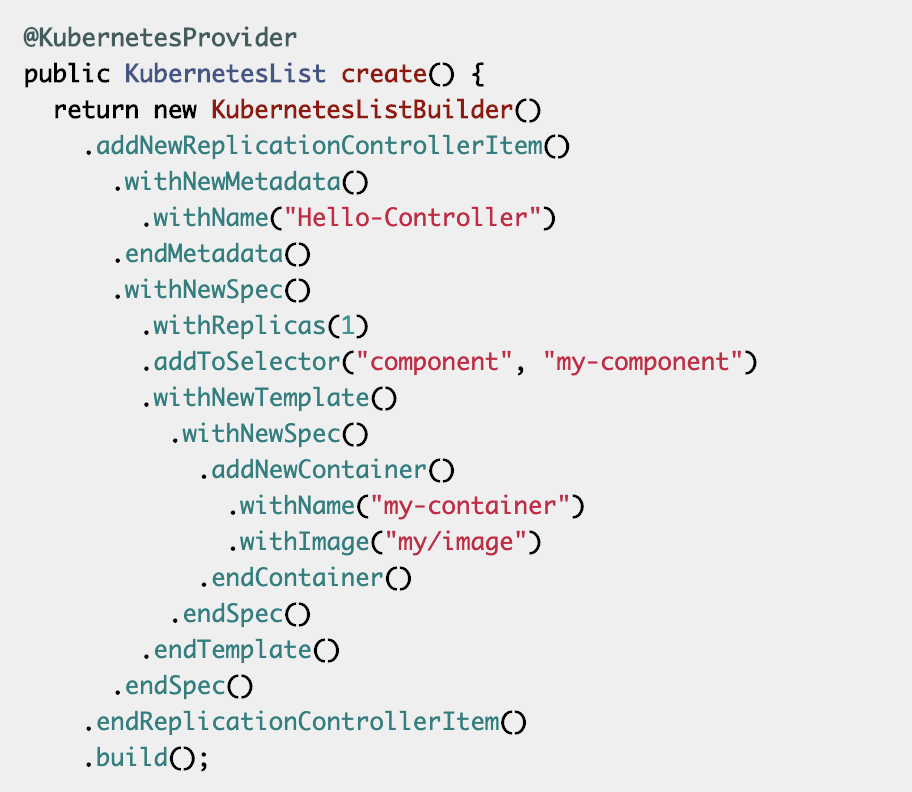
\includegraphics[height=5.8cm]{img/javamadness}
\end{minipage}
\end{textblock*}
\end{frame}

\begin{frame}{\ \ \ Кто, если не PHP?}
\setstretch{1.2}
\begin{textblock*}{\framewidth-0.8cm}(0.5cm,1.5cm)
\begin{itemize}
  \item На предыдущем слайде не PHP и не Pulumi, если что
  \item (а Java и fabric8.io)
\end{itemize}
\end{textblock*}
\end{frame}

\begin{frame}{\ \ \ Кто, если не PHP?}
\setstretch{1.2}
\begin{textblock*}{\framewidth-0.8cm}(0.5cm,1.5cm)
\begin{itemize}
  \item Ruby? Не думаю!
\end{itemize}
\begin{minipage}{\textwidth}
  \centering
  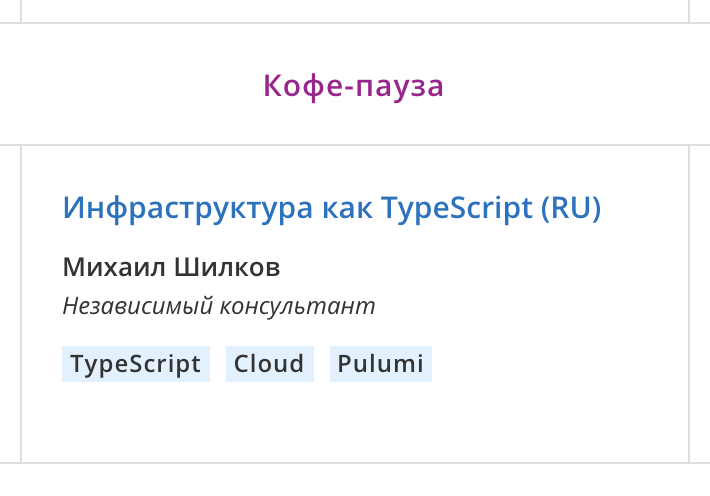
\includegraphics[height=5.8cm]{img/typescript}
\end{minipage}
\end{textblock*}
\end{frame}

\begin{frame}{\ \ \ K8s-only}
\setstretch{1.2}
\begin{textblock*}{\framewidth-0.8cm}(0.5cm,1.5cm)
\begin{itemize}
  \item Ksonnet (мертв)
  \item Jsonnet (жив, пахнет JSON-ом)
  \item Helm (жив, пахнет JSON-ом)
  \item Kustomize (жив, пахнет JSON-ом)
  \item k8s-kotlin-dsl
\end{itemize}
\end{textblock*}
\end{frame}

\begin{frame}{\ \ \ Kто там любил Ruby?}
\setstretch{1.2}
\begin{textblock*}{\framewidth-0.8cm}(0.5cm,1.5cm)
\begin{itemize}
  \item Хороший руби называется {\color {red}{\bf Kotlin}}
\end{itemize}
\begin{minipage}{\textwidth}
  \centering
  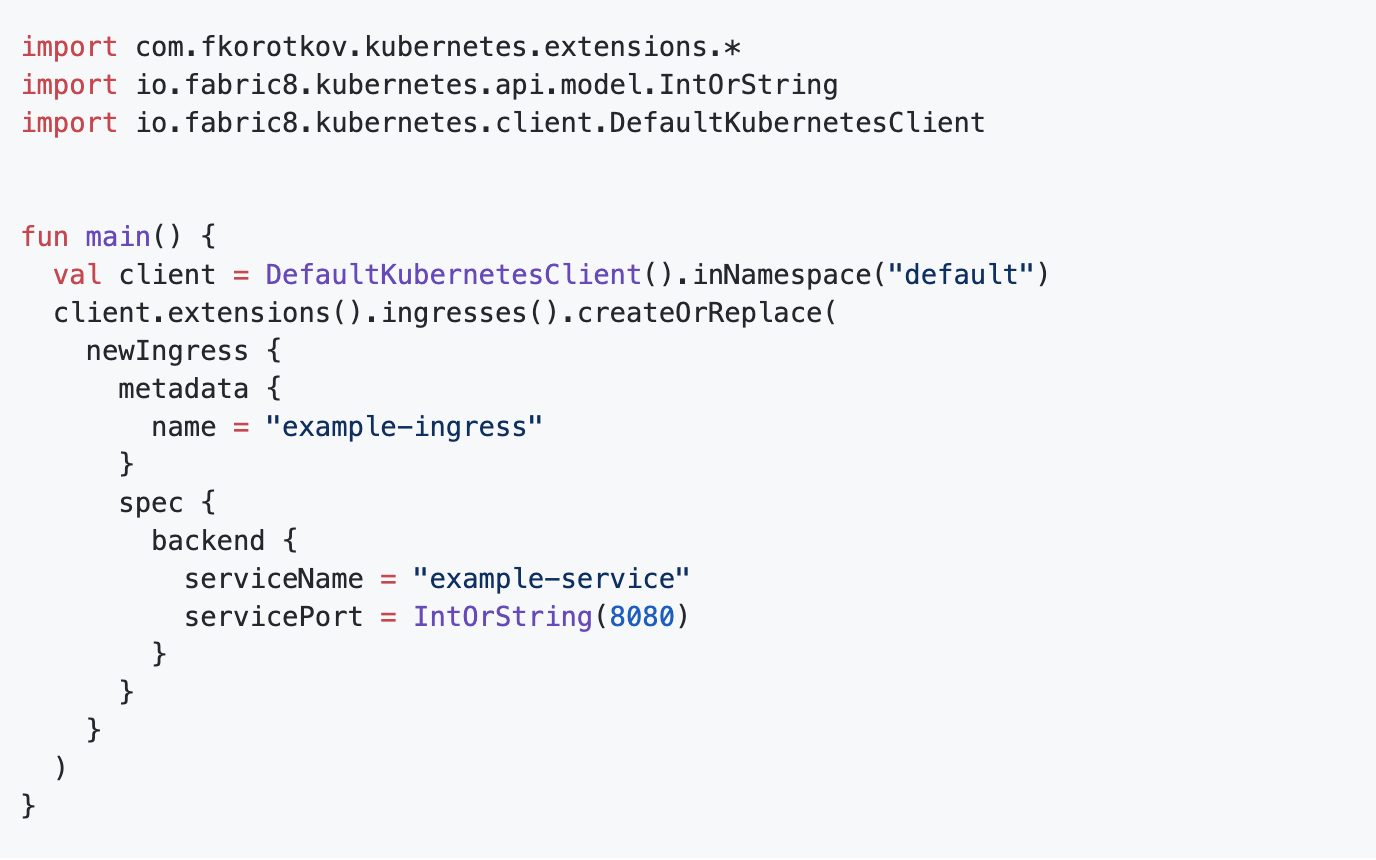
\includegraphics[height=6.2cm]{img/kotlindsl}
\end{minipage}
\end{textblock*}
\end{frame}

\begin{frame}{\ \ \ Харэ нас грузить!}
\setstretch{1.2}
\begin{textblock*}{\framewidth-0.8cm}(0.5cm,1.5cm)
\begin{itemize}
  \item Где практика?!.
\end{itemize}
\begin{minipage}{\textwidth}
  \centering
  
\includegraphics[height=5.8cm]{img/sooqah}
\end{minipage}
\end{textblock*}
\end{frame}

\begin{frame}{\ \ \ Практика}
\setstretch{1.2}
\begin{textblock*}{\framewidth-0.8cm}(0.5cm,1.5cm)
\begin{itemize}
  \item Весной 2018-го у нас уже был опыт
\end{itemize}
\end{textblock*}
\end{frame}

\begin{frame}{\ \ \ Практика}
\setstretch{1.2}
\begin{textblock*}{\framewidth-0.8cm}(0.5cm,1.5cm)
\begin{itemize}
  \item Весной 2018-го у нас уже был опыт
  \item Helm + Ansible (не спрашивайте!)
\end{itemize}
\end{textblock*}
\end{frame}

\begin{frame}{\ \ \ Почему Ansible}
\setstretch{1.2}
\begin{textblock*}{\framewidth-0.8cm}(0.5cm,1.5cm)
\begin{itemize}
  \item Огромное количество существующего опыта
\end{itemize}
\end{textblock*}
\end{frame}

\begin{frame}{\ \ \ Почему Ansible}
\setstretch{1.2}
\begin{textblock*}{\framewidth-0.8cm}(0.5cm,1.5cm)
\begin{itemize}
  \item Огромное количество существующего опыта
  \item Что угодно можно завернуть в роль Ansible
\end{itemize}
\end{textblock*}
\end{frame}

\begin{frame}{\ \ \ Почему Ansible}
\setstretch{1.2}
\begin{textblock*}{\framewidth-0.8cm}(0.5cm,1.5cm)
\begin{itemize}
  \item Огромное количество существующего опыта
  \item Что угодно можно завернуть в роль Ansible
  \item (Мы до сих пор так и делаем)
\end{itemize}
\end{textblock*}
\end{frame}

\begin{frame}{\ \ \ Почему Ansible}
\setstretch{1.2}
\begin{textblock*}{\framewidth-0.8cm}(0.5cm,1.5cm)
\begin{itemize}
  \item Огромное количество существующего опыта
  \item Что угодно можно завернуть в роль Ansible
  \item (Мы до сих пор так и делаем)
  \item Даже Helm!
\end{itemize}
\end{textblock*}
\end{frame}

\begin{frame}{\ \ \ Почему Ansible}
\setstretch{1.2}
\begin{textblock*}{\framewidth-0.8cm}(0.5cm,1.5cm)
\begin{itemize}
  \item Огромное количество существующего опыта
  \item Что угодно можно завернуть в роль Ansible
  \item (Мы до сих пор так и делаем)
  \item Даже Helm!
  \item \href{https://clck.ru/JfL3n}{\color{blue}{https://clck.ru/JfL3n}} (репа с лабой)
\end{itemize}
\end{textblock*}
\end{frame}

\begin{frame}{\ \ \ Что плохо в Helm}
\setstretch{1.2}
\begin{textblock*}{\framewidth-0.8cm}(0.5cm,1.5cm)
\begin{itemize}
  \item Внутри много все того же YAML
\end{itemize}
\end{textblock*}
\end{frame}

\begin{frame}{\ \ \ Что плохо в Helm}
\setstretch{1.2}
\begin{textblock*}{\framewidth-0.8cm}(0.5cm,1.5cm)
\begin{itemize}
  \item Внутри много все того же YAML
  \item (Нужно жить очень осторожно)
\end{itemize}
\end{textblock*}
\end{frame}

\begin{frame}{\ \ \ Что плохо в Helm}
\setstretch{1.2}
\begin{textblock*}{\framewidth-0.8cm}(0.5cm,1.5cm)
\begin{itemize}
  \item Внутри много все того же YAML
  \item (Нужно жить очень осторожно)
  \item Еще один шаблонизатор (сколько можно!)
\end{itemize}
\end{textblock*}
\end{frame}

\begin{frame}{\ \ \ Что плохо в Helm}
\setstretch{1.2}
\begin{textblock*}{\framewidth-0.8cm}(0.5cm,1.5cm)
\begin{itemize}
  \item Внутри много все того же YAML
  \item (Нужно жить очень осторожно)
  \item Еще один шаблонизатор (сколько можно!)
  \item В версии 2 есть k8s-сервис Tiller, работающий с правами кластерного админа
\end{itemize}
\end{textblock*}
\end{frame}

\begin{frame}{\ \ \ Что плохо не в Helm}
\setstretch{1.2}
\begin{textblock*}{\framewidth-0.8cm}(0.5cm,1.5cm)
\begin{itemize}
  \item Ни одна из проблем проекта не была связана с Helm
\end{itemize}
\end{textblock*}
\end{frame}

\begin{frame}{\ \ \ Что плохо не в Helm}
\setstretch{1.2}
\begin{textblock*}{\framewidth-0.8cm}(0.5cm,1.5cm)
\begin{itemize}
  \item Ни одна из проблем проекта не была связана с Helm
  \item Тяжело в России без нагана
\end{itemize}
\end{textblock*}
\end{frame}

\begin{frame}{\ \ \ Что очень хорошо в Helm}
\setstretch{1.2}
\begin{textblock*}{\framewidth-0.8cm}(0.5cm,1.5cm)
\begin{itemize}
  \item Helm потрясающе практичен
\end{itemize}
\end{textblock*}
\end{frame}

\begin{frame}{\ \ \ Что очень хорошо в Helm}
\setstretch{1.2}
\begin{textblock*}{\framewidth-0.8cm}(0.5cm,1.5cm)
\begin{itemize}
  \item Helm потрясающе практичен
  \item 340+ чартов в официальном репозитории
\end{itemize}
\end{textblock*}
\end{frame}

\begin{frame}{\ \ \ Что очень хорошо в Helm}
\setstretch{1.2}
\begin{textblock*}{\framewidth-0.8cm}(0.5cm,1.5cm)
\begin{itemize}
  \item Helm потрясающе практичен
  \item 340+ чартов в официальном репозитории
  \item Я немного занимаюсь open source, написать столько чартов у меня заняло
    бы 3+ года
\end{itemize}
\end{textblock*}
\end{frame}

\begin{frame}{\ \ \ Что будет дальше}
\setstretch{1.2}
\begin{textblock*}{\framewidth-0.8cm}(0.5cm,1.5cm)
\begin{itemize}
  \item Pulumi это проект CNCF
\end{itemize}
\end{textblock*}
\end{frame}

\begin{frame}{\ \ \ Что будет дальше}
\setstretch{1.2}
\begin{textblock*}{\framewidth-0.8cm}(0.5cm,1.5cm)
\begin{itemize}
  \item Pulumi это проект CNCF
  \item Подняли \$15M год назад
\end{itemize}
\end{textblock*}
\end{frame}

\begin{frame}{\ \ \ Что будет дальше}
\setstretch{1.2}
\begin{textblock*}{\framewidth-0.8cm}(0.5cm,1.5cm)
\begin{itemize}
  \item Pulumi это проект CNCF
  \item Подняли \$15M год назад
  \item И еще поднимут
\end{itemize}
\end{textblock*}
\end{frame}

\begin{frame}{\ \ \ Что будет дальше}
\setstretch{1.2}
\begin{textblock*}{\framewidth-0.8cm}(0.5cm,1.5cm)
\begin{itemize}
  \item Pulumi это проект CNCF
  \item Подняли \$15M год назад
  \item И все это надо вернуть
\end{itemize}
\end{textblock*}
\end{frame}

\begin{frame}{\ \ \ Что будет дальше}
\setstretch{1.2}
\begin{textblock*}{\framewidth-0.8cm}(0.5cm,1.5cm)
\begin{itemize}
  \item Pulumi это проект CNCF
  \item Подняли \$15M год назад
  \item И все это надо вернуть
  \item Я в первом ряду с попкорном
\end{itemize}
\end{textblock*}
\end{frame}

\begin{frame}{\ \ \ Что будет дальше}
\setstretch{1.2}
\begin{textblock*}{\framewidth-0.8cm}(0.5cm,1.5cm)
\begin{itemize}
  \item Два слова про Haskell и Python
\end{itemize}
\end{textblock*}
\end{frame}

\begin{frame}{\ \ \ Что будет дальше}
\setstretch{1.2}
\begin{textblock*}{\framewidth-0.8cm}(0.5cm,1.5cm)
\begin{itemize}
  \item Два слова про Haskell и Python
  \item Точнее, про Amazon, Stratosphere и Troposphere
\end{itemize}
\end{textblock*}
\end{frame}

\begin{frame}{\ \ \ Выводы}
\setstretch{1.2}
\begin{textblock*}{\framewidth-0.8cm}(0.5cm,1.5cm)
\begin{itemize}
  \item Туманно будущее
  \item Программисты на YAML еще будут нужны какое-то время
\end{itemize}
\end{textblock*}
\end{frame}

\begin{frame}{\ \ \ That's all, folks!}
\setstretch{1.2}
\begin{textblock*}{\framewidth-0.8cm}(0.5cm,1.5cm)
\begin{itemize}
  \item \href{mailto:alexclear@gmail.com}{\color{blue}{alexclear@gmail.com}}
  \item \href{https://telegram.me/lhommequipleure}{\color{blue}{https://telegram.me/lhommequipleure}}
  \item \href{https://telegram.me/demeliorator\_pod}{\color{blue}{https://telegram.me/demeliorator\_pod}}
\end{itemize}
\end{textblock*}
\end{frame}

\end{Large}

\end{document}
